\section{Dokumentacja techniczna codebase}

\subsection{Struktura repozytorium}
\begin{lstlisting}[style=reportcode]
Projekt_ADAC/
  backend/
    app/
      api/routes/            # endpointy FastAPI
      core/                  # konfiguracja, DB, logging
      models/                # ORM + schematy request/response
      repositories/          # dostep do danych
      services/              # feature engineering, policy, telemetry, trening danych
      ml/                    # trening i ewaluacja modelu
      scripts/               # seed i eksport replay
      tests/                 # testy jednostkowe
  frontend/
    src/
      api/                   # klient API
      components/            # testbed UI
      telemetry/             # collector + fingerprint + typy
  bot_runner/
    main.py                  # uruchamianie scenariuszy Playwright
    scenarios.py             # linear, human_like, adaptive, manual
  docker-compose.yml
  README.md
  raport/                    # dokumentacja LaTeX
\end{lstlisting}

\subsection{Frontend testbed (Vite + React + TypeScript)}
\subsubsection{Rola frontendu}
Frontend pelni podwojna funkcje:
\begin{itemize}
  \item \textbf{generatora naturalnych interakcji uzytkownika} (interfejs testowy),
  \item \textbf{sensora telemetrycznego} wysylajacego zdarzenia do backendu.
\end{itemize}

\subsubsection{Wyglad i funkcje interfejsu}
Widok frontendu pokazano na Rysunku~\ref{fig:frontend-ui}. Uklad ma trzy strefy:
\begin{itemize}
  \item \textbf{Panel sesji telemetrycznej} (gora): \texttt{session id}, liczniki eventow
  (\texttt{zbuforowane/wyslane}) i status collector pipeline.
  \item \textbf{Interaktywny testbed ruchu} (lewa kolumna): menu, wyszukiwarka,
  filtry kategorii, karty produktowe i przyciski CTA. To celowo przypomina
  realistyczny scenariusz e-commerce.
  \item \textbf{Silnik ochrony} (prawa kolumna): uruchamianie predykcji, reczne
  etykietowanie sesji (\texttt{human}/\texttt{bot}) i podglad wyniku:
  \texttt{risk score}, \texttt{predykcja}, \texttt{confidence}, \texttt{decyzja}.
\end{itemize}

\begin{figure}[H]
  \centering
  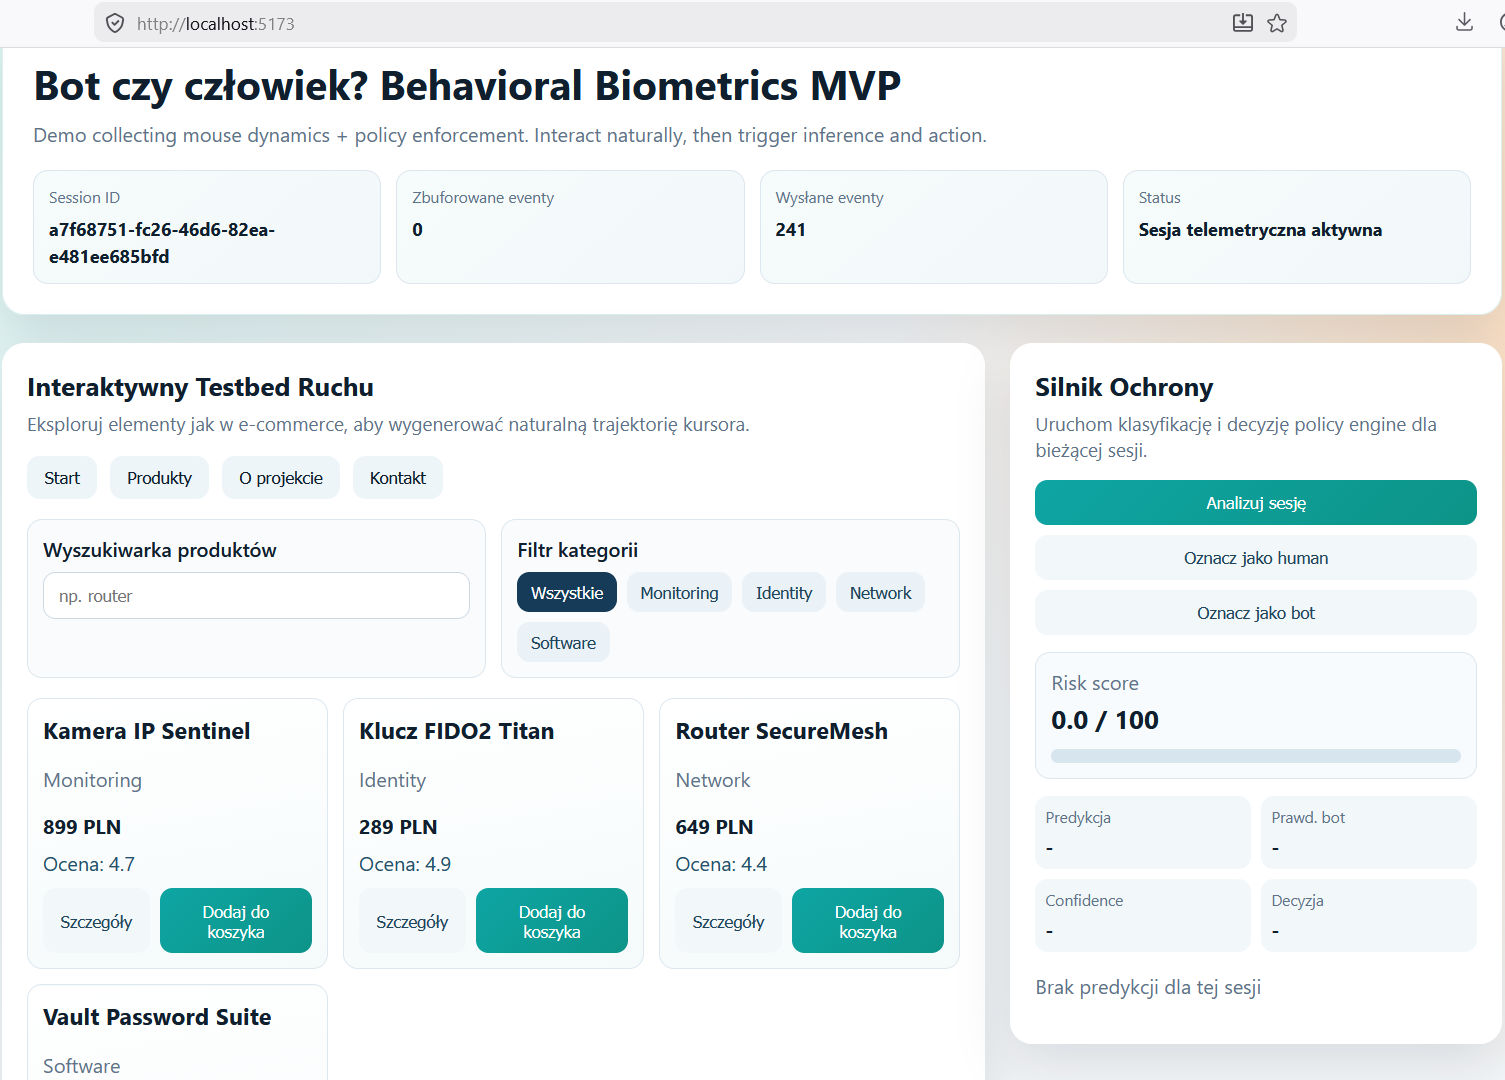
\includegraphics[width=0.98\textwidth]{frontend_view.png}
  \caption{Frontend testbed na localhost: panel telemetryczny, strefa interakcji i panel policy engine}
  \label{fig:frontend-ui}
\end{figure}

\subsubsection{Zbierane eventy i batching}
Kolektor (\texttt{frontend/src/telemetry/collector.ts}) rejestruje:
\begin{itemize}
  \item \texttt{mousemove},
  \item \texttt{click},
  \item \texttt{scroll},
  \item \texttt{focus},
  \item \texttt{blur},
  \item \texttt{viewport\_enter}/\texttt{viewport\_leave}
  (przez \texttt{visibilitychange}).
\end{itemize}

Wysylka odbywa sie partiami:
\begin{itemize}
  \item \texttt{batchSize = 35},
  \item okresowe \texttt{flush} co \texttt{2000 ms},
  \item retry: eventy wracaja do bufora przy bledzie API.
\end{itemize}

\subsubsection{Fingerprint klienta}
Zbierane cechy srodowiskowe obejmuja m.in.:
\begin{itemize}
  \item \texttt{user\_agent}, \texttt{language}, \texttt{timezone},
  \item \texttt{screen\_width/height}, \texttt{viewport\_width/height},
  \item \texttt{platform}, \texttt{pointer\_type},
  \item \texttt{webdriver}, \texttt{headless\_hint},
  \item \texttt{hardware\_concurrency}, \texttt{device\_memory}.
\end{itemize}

\subsection{Pozyskanie danych treningowych (human vs bot)}
\subsubsection{Jak zbierano dane klasy human}
Dane \texttt{human} byly zbierane manualnie przez interakcje operatora z frontendem
(Rysunek~\ref{fig:frontend-ui}): ruch myszy po menu, filtrach i kartach,
klikniecia, scrollowanie i wpisywanie fraz w wyszukiwarce.
Po zakonczonej probce sesje oznaczano przyciskiem \texttt{Oznacz jako human}.

\subsubsection{Jak zbierano dane klas botowych}
Sesje botowe generowano automatycznie przez \texttt{bot\_runner}:
\begin{lstlisting}[style=reportcode]
docker compose exec bot_runner python main.py --scenario linear --sessions 25 --record-video
docker compose exec bot_runner python main.py --scenario human_like --sessions 26 --record-video
docker compose exec bot_runner python main.py --scenario adaptive --sessions 50 --record-video
\end{lstlisting}

\subsubsection{Udzial scenariuszy botowych}
Na poziomie sesji botowych przyjeto:
\begin{itemize}
  \item \texttt{linear}: 25 sesji (24.75\% klasy bot),
  \item \texttt{human\_like}: 26 sesji (25.74\% klasy bot),
  \item \texttt{adaptive}: 50 sesji (49.50\% klasy bot).
\end{itemize}
Lacznie: 101 sesji botowych.

\subsubsection{Charakterystyka botow i zamysl projektowy}
\begin{itemize}
  \item \texttt{linear}: ruch prosty i rytmiczny, niski realizm.
  Cel: latwy baseline wykrywania prostych automatyzacji.
  \item \texttt{human\_like}: krzywe Beziera, jitter i losowe opoznienia.
  Cel: etap posredni pomiedzy botem prostym i trudniejszym.
  \item \texttt{adaptive}: scenariusz kalibrowany profilem zachowan czlowieka
  (\texttt{/api/v1/sessions/human-behavior-profile}), z dynamicznym tempem ruchu,
  pauzami, korektami toru i bardziej realistycznym typingiem.
  Cel: utrudnic klasyfikacje i przetestowac odpornosc modelu na boty
  zblizone dystrybucyjnie do klasy \texttt{human}.
\end{itemize}

\subsection{Backend Collector API (FastAPI)}
\subsubsection{Warstwy backendu}
\begin{itemize}
  \item \textbf{API routes} -- walidacja wejscia/wyjscia (Pydantic) i kontrakty REST.
  \item \textbf{Services} -- logika domenowa (telemetria, cechy, polityki, model).
  \item \textbf{Repositories} -- operacje bazodanowe (SQLAlchemy ORM).
  \item \textbf{ML module} -- trening i ewaluacja modelu.
\end{itemize}

\subsubsection{Endpointy REST}
\begin{longtable}{
  >{\ttfamily\footnotesize\raggedright\arraybackslash}p{0.47\textwidth}
  @{\hspace{1.0em}}
  >{\centering\arraybackslash}p{0.09\textwidth}
  @{\hspace{0.8em}}
  >{\raggedright\arraybackslash}p{0.32\textwidth}
}
\toprule
\textnormal{Endpoint} & \textnormal{Metoda} & \textnormal{Opis} \\
\midrule
\endhead
\textnormal{/api/v1/health} & GET & Healthcheck aplikacji. \\
\textnormal{/api/v1/sessions} & POST & Utworzenie nowej sesji i zapis fingerprintu. \\
\textnormal{/api/v1/events/batch} & POST & Przyjecie batcha eventow dla sesji. \\
\textnormal{/api/v1/sessions/\{session\_id\}/label} & POST & Etykietowanie sesji jako \texttt{human} lub \texttt{bot}. \\
\textnormal{/api/v1/predict/\{session\_id\}} & POST & Predykcja dla sesji + decyzja policy engine. \\
\textnormal{/api/v1/predictions/\{session\_id\}} & GET & Pobranie ostatniej predykcji sesji. \\
\textnormal{/api/v1/sessions/\{session\_id\}} & GET & Status sesji i metadane. \\
\textnormal{/api/v1/sessions/human-behavior-profile} & GET & Profil statystyczny zachowan czlowieka do adaptacji bota. \\
\bottomrule
\end{longtable}

\subsection{Storage: PostgreSQL}
Model danych sklada sie z pieciu tabel:
\begin{itemize}
  \item \texttt{sessions} -- glowna encja sesji,
  \item \texttt{raw\_events} -- surowy strumien interakcji,
  \item \texttt{predictions} -- wyniki modelu,
  \item \texttt{model\_versions} -- rejestr wersji modelu i metryk,
  \item \texttt{enforcement\_actions} -- decyzje polityki ochronnej.
\end{itemize}

Relacje opisuje diagram ERD w Sekcji 2.

\subsection{Slownik zmiennych bazodanowych}
Tabela~\ref{tab:db-variable-dictionary} pokazuje wszystkie zmienne przechowywane
w bazie PostgreSQL. Kolumna \texttt{czy wchodzi do modelu} oznacza, czy dana
zmienna jest wykorzystywana w pipeline cech (bezposrednio lub przez transformacje).

\begin{longtable}{
  >{\ttfamily\scriptsize\raggedright\arraybackslash\hspace{0pt}}p{0.33\textwidth}
  @{\hspace{1.0em}}
  >{\footnotesize\raggedright\arraybackslash}p{0.52\textwidth}
  @{\hspace{0.8em}}
  >{\footnotesize\centering\arraybackslash}p{0.06\textwidth}
}
\caption{Slownik zmiennych bazodanowych: znaczenie i udzial w modelu}
\label{tab:db-variable-dictionary} \\
\toprule
\textnormal{nazwa\_zmiennej} & \textnormal{co zmienna oznacza (jak jest wyliczana)} & \textnormal{czy wchodzi do modelu} \\
\midrule
\endfirsthead
\toprule
\textnormal{nazwa\_zmiennej} & \textnormal{co zmienna oznacza (jak jest wyliczana)} & \textnormal{czy wchodzi do modelu} \\
\midrule
\endhead
\textnormal{sessions.id} & identyfikator sesji (UUID). & NIE \\
\textnormal{sessions.source} & zrodlo sesji (np. \texttt{frontend} / \texttt{bot\_runner}). & NIE \\
\textnormal{sessions.true\_label} & etykieta referencyjna \texttt{human}/\texttt{bot} nadawana recznie lub automatycznie. & NIE \\
\textnormal{sessions.status} & status procesu sesji (np. collecting, predicted). & NIE \\
\textnormal{sessions.client\_fingerprint} & surowy fingerprint klienta (JSON). & NIE \\
\textnormal{sessions.environment} & surowe parametry srodowiskowe (JSON), zrodlo cech srodowiskowych. & TAK \\
\textnormal{sessions.created\_at} & czas utworzenia rekordu sesji. & NIE \\
\textnormal{sessions.updated\_at} & czas ostatniej aktualizacji sesji. & NIE \\
\textnormal{sessions.environment.user\_agent} & identyfikator przegladarki/OS; uzywany do flag pomocniczych. & TAK \\
\textnormal{sessions.environment.language} & jezyk przegladarki. & NIE \\
\textnormal{sessions.environment.timezone} & strefa czasowa klienta. & NIE \\
\textnormal{sessions.environment.screen\_width} & szerokosc ekranu klienta; skladnik \texttt{screen\_area}. & TAK \\
\textnormal{sessions.environment.screen\_height} & wysokosc ekranu klienta; skladnik \texttt{screen\_area}. & TAK \\
\textnormal{sessions.environment.viewport\_width} & szerokosc viewportu; skladnik \texttt{viewport\_area}. & TAK \\
\textnormal{sessions.environment.viewport\_height} & wysokosc viewportu; skladnik \texttt{viewport\_area}. & TAK \\
\textnormal{sessions.environment.webdriver} & flaga automatyzacji przegladarki. & TAK \\
\textnormal{sessions.environment.headless\_hint} & sygnal trybu headless. & TAK \\
\textnormal{sessions.environment.hardware\_concurrency} & liczba logicznych rdzeni CPU raportowana przez przegladarke. & TAK \\
\textnormal{sessions.environment.device\_memory} & pamiec urzadzenia raportowana przez przegladarke. & TAK \\
\textnormal{raw\_events.id} & techniczny identyfikator eventu. & NIE \\
\textnormal{raw\_events.session\_id} & klucz obcy do sesji. & NIE \\
\textnormal{raw\_events.sequence\_no} & numer sekwencyjny eventu w batchu. & NIE \\
\textnormal{raw\_events.event\_type} & typ eventu (\texttt{mousemove}, \texttt{click}, \texttt{scroll}, ...). & TAK \\
\textnormal{raw\_events.ts\_ms} & timestamp eventu w milisekundach, baza do dynamiki. & TAK \\
\textnormal{raw\_events.x} & pozycja X kursora. & TAK \\
\textnormal{raw\_events.y} & pozycja Y kursora. & TAK \\
\textnormal{raw\_events.scroll\_x} & przesuniecie poziome scrolla. & NIE \\
\textnormal{raw\_events.scroll\_y} & przesuniecie pionowe scrolla, baza \texttt{scroll\_velocity}. & TAK \\
\textnormal{raw\_events.target\_id} & identyfikator celu eventu; baza \texttt{hover/target\_revisit}. & TAK \\
\textnormal{raw\_events.target\_tag} & tag HTML celu interakcji. & NIE \\
\textnormal{raw\_events.target\_class} & klasy CSS celu interakcji. & NIE \\
\textnormal{raw\_events.pointer\_type} & typ urzadzenia wskazujacego. & NIE \\
\textnormal{raw\_events.in\_viewport} & flaga widocznosci eventu w viewport. & NIE \\
\textnormal{raw\_events.payload} & dodatkowy payload zdarzenia (JSON). & NIE \\
\textnormal{raw\_events.created\_at} & czas zapisu eventu. & NIE \\
\textnormal{predictions.id} & identyfikator predykcji. & NIE \\
\textnormal{predictions.session\_id} & sesja, dla ktorej wykonano predykcje. & NIE \\
\textnormal{predictions.model\_version\_id} & wersja modelu uzyta do inferencji. & NIE \\
\textnormal{predictions.predicted\_label} & wynik klasyfikacji modelu (\texttt{human}/\texttt{bot}). & NIE \\
\textnormal{predictions.probability\_bot} & prawdopodobienstwo klasy \texttt{bot}. & NIE \\
\textnormal{predictions.confidence} & pewnosc predykcji (maksimum prawdopodobienstwa). & NIE \\
\textnormal{predictions.risk\_score} & przeskalowany wynik ryzyka 0--100. & NIE \\
\textnormal{predictions.feature\_snapshot} & snapshot wektora cech wykorzystanych przy predykcji. & NIE \\
\textnormal{predictions.created\_at} & czas utworzenia predykcji. & NIE \\
\textnormal{model\_versions.id} & identyfikator wersji modelu. & NIE \\
\textnormal{model\_versions.name} & nazwa modelu. & NIE \\
\textnormal{model\_versions.version} & oznaczenie wersji (np. timestamp). & NIE \\
\textnormal{model\_versions.algorithm} & algorytm (Decision Tree). & NIE \\
\textnormal{model\_versions.feature\_set\_version} & wersja zestawu cech. & NIE \\
\textnormal{model\_versions.metrics} & metryki treningowe/ewaluacyjne (JSON). & NIE \\
\textnormal{model\_versions.artifact\_path} & sciezka do artefaktu modelu. & NIE \\
\textnormal{model\_versions.model\_metadata} & metadane modelu (JSON). & NIE \\
\textnormal{model\_versions.is\_active} & flaga aktywnej wersji modelu. & NIE \\
\textnormal{model\_versions.created\_at} & czas rejestracji wersji modelu. & NIE \\
\textnormal{enforcement\_actions.id} & identyfikator decyzji polityki. & NIE \\
\textnormal{enforcement\_actions.session\_id} & sesja, ktorej dotyczy decyzja. & NIE \\
\textnormal{enforcement\_actions.prediction\_id} & predykcja powiazana z decyzja. & NIE \\
\textnormal{enforcement\_actions.action} & decyzja (\texttt{allow}/\texttt{observe}/\texttt{throttle}/\texttt{challenge}/\texttt{block}). & NIE \\
\textnormal{enforcement\_actions.reason} & uzasadnienie decyzji polityki. & NIE \\
\textnormal{enforcement\_actions.blocked\_until} & koniec blokady czasowej (jesli dotyczy). & NIE \\
\textnormal{enforcement\_actions.action\_metadata} & dodatkowe metadane decyzji (JSON). & NIE \\
\textnormal{enforcement\_actions.created\_at} & czas zapisu decyzji. & NIE \\
\bottomrule
\end{longtable}

\subsection{Feature engineering}
Pipeline cech (\texttt{backend/app/services/feature\_engineering.py}) liczy cechy
z okna eventow posortowanych po czasie (\texttt{ts\_ms}), a nie z pojedynczego eventu.

\subsubsection{Przykladowe cechy dynamiczne}
\begin{itemize}
  \item trajektoria i geometria: \texttt{path\_length}, \texttt{displacement}, \texttt{path\_efficiency},
  \item dynamika ruchu: \texttt{speed\_mean/std/max}, \texttt{acc\_mean/std/max}, \texttt{jerk\_mean/std/max},
  \item mikrozachowania: \texttt{micro\_pause\_count}, \texttt{correction\_rhythm}, \texttt{overshoot\_count},
  \item klikniecia: \texttt{click\_interval\_mean/std}, \texttt{hover\_before\_click\_mean}, \texttt{target\_revisit\_count},
  \item kontekst sekwencji: \texttt{event\_type\_entropy}, \texttt{unique\_event\_types},
  \item scroll i focus: \texttt{scroll\_velocity\_mean/std}, \texttt{focus\_blur\_transitions}.
\end{itemize}

\subsubsection{Cechy srodowiskowe}
Pipeline zawiera takze cechy srodowiskowe, jednak w finalnym modelu drzewa
sa one \textbf{domyslnie wylaczone z treningu} (\texttt{feature\_set=behavioral}),
aby ograniczyc ryzyko data leakage (np. trywialny podzial po \texttt{viewport\_area}).

\subsubsection{Slownik zmiennych cechowych}
Tabela~\ref{tab:feature-dictionary} zawiera komplet zmiennych cechowych budowanych
w pipeline i informacje, czy dana zmienna wchodzi do finalnego modelu.

\begin{longtable}{
  >{\ttfamily\scriptsize\raggedright\arraybackslash\hspace{0pt}}p{0.27\textwidth}
  @{\hspace{1.0em}}
  >{\footnotesize\raggedright\arraybackslash}p{0.57\textwidth}
  @{\hspace{0.8em}}
  >{\footnotesize\centering\arraybackslash}p{0.06\textwidth}
}
\caption{Slownik zmiennych cechowych: nazwa, znaczenie i uzycie w modelu finalnym}
\label{tab:feature-dictionary} \\
\toprule
\textnormal{nazwa\_zmiennej} & \textnormal{co zmienna oznacza (jak jest wyliczana)} & \textnormal{czy wchodzi do modelu} \\
\midrule
\endfirsthead
\toprule
\textnormal{nazwa\_zmiennej} & \textnormal{co zmienna oznacza (jak jest wyliczana)} & \textnormal{czy wchodzi do modelu} \\
\midrule
\endhead
\textnormal{event\_count} & liczba wszystkich eventow w oknie czasowym. & TAK \\
\textnormal{window\_duration\_ms} & czas trwania okna: \texttt{ts\_last - ts\_first}. & TAK \\
\textnormal{mousemove\_count} & liczba eventow \texttt{mousemove}. & TAK \\
\textnormal{click\_count} & liczba eventow \texttt{click}. & TAK \\
\textnormal{scroll\_count} & liczba eventow \texttt{scroll}. & TAK \\
\textnormal{focus\_blur\_transitions} & suma liczby eventow \texttt{focus} i \texttt{blur}. & TAK \\
\textnormal{viewport\_enter\_count} & liczba eventow \texttt{viewport\_enter}. & TAK \\
\textnormal{viewport\_leave\_count} & liczba eventow \texttt{viewport\_leave}. & TAK \\
\textnormal{path\_length} & suma odleglosci euklidesowych pomiedzy kolejnymi punktami kursora. & TAK \\
\textnormal{displacement} & odleglosc miedzy pierwszym i ostatnim punktem kursora w oknie. & TAK \\
\textnormal{path\_efficiency} & wspolczynnik \texttt{displacement / max(path\_length, 1)}. & TAK \\
\textnormal{speed\_mean} & srednia predkosc kursora pomiedzy kolejnymi punktami (\texttt{distance/dt}). & TAK \\
\textnormal{speed\_std} & odchylenie standardowe predkosci kursora. & TAK \\
\textnormal{speed\_max} & maksymalna predkosc kursora w oknie. & TAK \\
\textnormal{acc\_mean} & srednie przyspieszenie: \texttt{delta(speed)/dt}. & TAK \\
\textnormal{acc\_std} & odchylenie standardowe przyspieszenia. & TAK \\
\textnormal{acc\_max} & maksymalne przyspieszenie w oknie. & TAK \\
\textnormal{jerk\_mean} & sredni jerk: \texttt{delta(acc)/dt}. & TAK \\
\textnormal{jerk\_std} & odchylenie standardowe jerk. & TAK \\
\textnormal{jerk\_max} & maksymalny jerk w oknie. & TAK \\
\textnormal{curvature\_mean} & srednia krzywizna toru: \texttt{|delta(kat)| / max(distance, 1)}. & TAK \\
\textnormal{curvature\_std} & odchylenie standardowe krzywizny toru. & TAK \\
\textnormal{angle\_change\_mean} & srednia zmiana kata ruchu pomiedzy kolejnymi segmentami. & TAK \\
\textnormal{angle\_change\_std} & odchylenie standardowe zmian kata ruchu. & TAK \\
\textnormal{micro\_pause\_count} & liczba segmentow z bardzo niska predkoscia (\texttt{speed < 40 px/s}). & TAK \\
\textnormal{correction\_rhythm} & liczba mocnych korekt kierunku (prog zmiany kata \texttt{> 1.1 rad}). & TAK \\
\textnormal{click\_interval\_mean} & sredni odstep czasowy miedzy kolejnymi kliknieciami. & TAK \\
\textnormal{click\_interval\_std} & odchylenie standardowe odstepow miedzy kliknieciami. & TAK \\
\textnormal{hover\_before\_click\_mean} & sredni czas hover przed kliknieciem, liczony lokalnie przy celu klikniecia. & TAK \\
\textnormal{dwell\_time\_mean} & sredni czas przebywania na segmentach (\texttt{1000/max(speed,1)}). & TAK \\
\textnormal{overshoot\_count} & liczba przypadkow overshoot (rewersy kierunku przed kliknieciem). & TAK \\
\textnormal{target\_revisit\_count} & liczba celow klikanych wielokrotnie w tej samej sesji okna. & TAK \\
\textnormal{scroll\_velocity\_mean} & srednia predkosc scrolla: \texttt{|delta(scroll\_y)|/dt}. & TAK \\
\textnormal{scroll\_velocity\_std} & odchylenie standardowe predkosci scrolla. & TAK \\
\textnormal{unique\_event\_types} & liczba unikalnych typow eventow w oknie. & TAK \\
\textnormal{event\_type\_entropy} & entropia Shannona rozkladu typow eventow w oknie. & TAK \\
\textnormal{webdriver\_flag} & flaga 0/1: czy \texttt{navigator.webdriver} jest prawda. & NIE \\
\textnormal{headless\_flag} & flaga 0/1: wykrycie sygnalu headless na podstawie \texttt{user-agent}. & NIE \\
\textnormal{viewport\_area} & pole viewportu: \texttt{viewport\_width * viewport\_height}. & NIE \\
\textnormal{screen\_area} & pole ekranu: \texttt{screen\_width * screen\_height}. & NIE \\
\textnormal{viewport\_screen\_ratio} & iloraz \texttt{viewport\_area / max(screen\_area,1)}. & NIE \\
\textnormal{hardware\_concurrency} & liczba logicznych rdzeni CPU raportowana przez przegladarke. & NIE \\
\textnormal{device\_memory} & pamiec urzadzenia raportowana przez przegladarke. & NIE \\
\bottomrule
\end{longtable}

\subsection{Model i inferencja}
\subsubsection{Trening offline}
Skrypt \texttt{python -m app.ml.train} realizuje:
\begin{itemize}
  \item budowe DataFrame z okien (\texttt{window\_size}, \texttt{stride}),
  \item podzial train/test z grupowaniem po \texttt{session\_id} (\texttt{GroupShuffleSplit}),
  \item trening \texttt{DecisionTreeClassifier} z \texttt{class\_weight=balanced},
  \item zapis artefaktow: model, metryki, ROC, confusion matrix, drzewo i reguly.
\end{itemize}

\subsubsection{Predykcja online}
Inferencja dziala przez \texttt{ModelManager}:
\begin{itemize}
  \item laduje aktywny artefakt modelu (\texttt{active\_model.joblib}),
  \item zwraca \texttt{predicted\_label}, \texttt{probability\_bot}, \texttt{confidence}, \texttt{risk\_score},
  \item przy braku modelu uzywa fallbacku heurystycznego.
\end{itemize}

\subsection{Policy engine / enforcement}
Mapowanie ryzyka (\texttt{backend/app/services/policy\_engine.py}):
\begin{itemize}
  \item \texttt{risk < 25}: \texttt{allow},
  \item \texttt{25--50}: \texttt{observe},
  \item \texttt{50--75}: \texttt{throttle},
  \item \texttt{75--90}: \texttt{challenge},
  \item \texttt{>= 90}: \texttt{block}.
\end{itemize}

\subsection{DevOps i uruchomienie}
Srodowisko dziala lokalnie przez Docker Compose:
\begin{itemize}
  \item \texttt{frontend} -- port 5173,
  \item \texttt{backend} -- port 8000,
  \item \texttt{db} -- port 5432,
  \item \texttt{bot\_runner} -- kontener narzedziowy do generacji sesji.
\end{itemize}

\subsection{Jakosc i testy}
\begin{itemize}
  \item testy jednostkowe backendu (\texttt{backend/app/tests}),
  \item walidacja kontraktow API przez schematy Pydantic,
  \item separacja odpowiedzialnosci: API/Services/Repositories/ML.
\end{itemize}

